\chapter{Families of Groups}
\label{chapter:families}
\thispagestyle{empty}

In this chapter we will explore a few families of groups, some of which we are already familiar with.

\begin{section}{Cyclic Groups}

Recall that if $G$ is a group and $g\in G$, then the \textbf{cyclic subgroup generated by $g$} is given by
\[
\langle g\rangle =\{g^k\mid k\in\mathbb{Z}\}.
\]
It is important to point out that $\langle g\rangle$ may be finite or infinite. In the finite case, the Cayley diagram with generator $g$ gives us a good indication of where the word ``cyclic" comes from (see Problem~\ref{prob:Cayley_cyclic}).  If there exists $g\in G$ such that $G=\langle g\rangle$, then we say that $G$ is a \textbf{cyclic group}.  

\begin{problem}
List all of the elements in each of the following cyclic subgroups.
\begin{enumerate}[label=\rm{(\alph*)}]
\item $\langle r\rangle$, where $r\in D_3$
\item $\langle r\rangle$, where $r\in R_4$
\item $\langle rs\rangle$, where $rs\in D_4$
\item $\langle r^2\rangle$, where $r^2\in R_6$
\item $\langle i\rangle$, where $i\in Q_8$
\item $\langle 6\rangle$, where $6\in \mathbb{Z}$ and the operation is ordinary addition
\end{enumerate}
\end{problem}

\begin{problem}\label{prob:subgroup_generated_by_matrix}
Consider the group of invertible $2\times 2$ matrices with real number entries under the operation of matrix multiplication.  This group is denoted by $\mathrm{GL}_2(\mathbb{R})$.  List the elements in the cyclic subgroups generated by each of the following matrices.
\begin{multicols}{3}
\begin{enumerate}[label=\rm{(\alph*)}]
\item $\begin{bmatrix} 0 & -1\\ -1 & 0\end{bmatrix}$
\item $\begin{bmatrix} 0 & -1\\ 1 & 0\end{bmatrix}$
\item $\begin{bmatrix} 2 & 0\\ 0 & 1\end{bmatrix}$
\end{enumerate}
\end{multicols}
\end{problem}

\begin{problem}\label{prob:cyclic_or_not}
Determine whether each of the following groups is cyclic.  
%Determine whether each of the groups from Problem~\ref{prob:computing_orders} is cyclic.
If the group is cyclic, find at least one generator.
\begin{multicols}{2}
\begin{enumerate}[label=\rm{(\alph*)}]
\item $S_2$
\item $R_3$
\item $R_4$
\item $V_4$
\item $R_5$
\item $R_6$
\item $D_3$
\item $R_7$
\item $R_8$
\item $\Spin_{1\times 2}$
\item $D_4$
\item $Q_8$
\end{enumerate}
\end{multicols}
\end{problem}

\begin{problem}
Determine whether each of the following groups is cyclic.  If the group is cyclic, find at least one generator. If you believe that a group is not cyclic, try to sketch an argument.
\begin{multicols}{2}
\begin{enumerate}[label=\rm{(\alph*)}]
\item $(\mathbb{Z},+)$
\item $(\mathbb{R},+)$
\item $(\mathbb{R}^+,\cdot)$
\item $(\{6^n\mid n\in\mathbb{Z}\},\cdot)$
\end{enumerate}
\end{multicols}
\begin{enumerate}
\item[(e)] $\textrm{GL}_2(\mathbb{R})$ under matrix multiplication
\item[(f)] $\{(\cos(\pi/4) +i\sin(\pi/4))^n\mid n\in \mathbb{Z}\}$ under multiplication of complex numbers
\end{enumerate}
\end{problem}

\begin{theorem}\label{thm:cyclic_implies_abelian}
If $G$ is a cyclic group, then $G$ is abelian.
\end{theorem}

\begin{problem}\label{prob:abelian_does_not_imply_cyclic}
Provide an example of a finite group that is abelian but not cyclic.
\end{problem}

\begin{problem}
Provide an example of an infinite group that is abelian but not cyclic.
\end{problem}

\begin{theorem}\label{thm:subgroup_generated_by_inverse}
If $G$ is a group and $g\in G$, then $\langle g\rangle=\langle g^{-1}\rangle$.
\end{theorem}

\begin{theorem}
If $G$ is a cyclic group such that $G$ has exactly one element that generates all of $G$, then the order of $G$ is at most order 2.   
\end{theorem}

\begin{theorem}
If $G$ is a group such that $G$ has no proper nontrivial subgroups, then $G$ is cyclic.
\end{theorem}

Recall that the order of a group $G$, denoted $|G|$, is the number of elements in $G$. We define the \textbf{order} of an element $g$, written $|g|$, to be the order of $\langle g\rangle$.  That is, $|g|=|\langle g\rangle|$.  It is clear that $G$ is cyclic with generator $g$ if and only if $|G|=|g|$.

\begin{problem}
What is the order of the identity in any group?
\end{problem}

\begin{problem}\label{prob:computing_orders}
Find the orders of each of the elements in each of the groups in Problem~\ref{prob:cyclic_or_not}.
\end{problem}

\begin{problem}
Consider the group $(\mathbb{Z},+)$.  What is the order of 1?  Are there any elements in $\mathbb{Z}$ with finite order?
\end{problem}

\begin{problem}
Find the order of each of the matrices in Problem~\ref{prob:subgroup_generated_by_matrix}.
\end{problem}

The next result follows immediately from Theorem~\ref{thm:subgroup_generated_by_inverse}.

\begin{theorem}
If $G$ is a group and $g\in G$, then $|g|=|g^{-1}|$.
\end{theorem}

The next result should look familiar and will come in handy a few times in this chapter. We'll take the result for granted and not worry about proving it.

\begin{theorem}[Division Algorithm]
If $n$ is a positive integer and $m$ is any integer, then there exist unique integers $q$ (called the \textbf{quotient}) and $r$ (called the \textbf{remainder}) such that $m=nq+r$, where $0\leq r<n$.
\end{theorem}

\begin{theorem}\label{thm:finite_group_finite_exponent}
Suppose $G$ is a group and let $g\in G$. The subgroup $\langle g\rangle$ is finite if and only if there exists $n\in\mathbb{N}$ such that $g^n=e$.\footnote{For the forward implication, if $\langle g\rangle$ is finite, then there exists distinct positive integers $i$ and $j$ such that $g^i=g^j$.  Can you find a useful way to rewrite this equation? For the reverse implication, let $m\in\mathbb{Z}$ and use the Division Algorithm with $m$ and $n$.}
\end{theorem}

\begin{corollary}\label{cor:finite_group_finite_exponent}
If $G$ is a finite group, then for all $g\in G$, there exists $n\in\mathbb{N}$ such that $g^n=e$.
\end{corollary}

\begin{theorem}
Suppose $G$ is a group and let $g\in G$ such that $\langle g\rangle$ is a finite group. If $n$ is the smallest positive integer such that $g^n=e$, then $\langle g\rangle = \{e, g, g^2, \ldots, g^{n-1}\}$ and this set contains $n$ distinct elements.\footnote{Note that Theorem~\ref{thm:finite_group_finite_exponent} together with the Well-Ordering Principle guarantees the existence of a smallest positive integer $n$ such that $g^n=e$. The claim that the set contains $n$ distinct elements is not immediate.  You need to argue that there are no repeats in the list. Choose distinct $i,j\in\{0,1,\ldots,n-1\}$ such that $i\neq j$ and then show that $g^i\neq g^j$.  Consider a proof by contradiction and try to contradict the minimality of $n$.}
\end{theorem}

The next result provides an extremely useful interpretation of the order of an element.

\begin{corollary}\label{cor:order_smallest_exponent}
If $G$ is a group and $g\in G$ such that $\langle g\rangle$ is a finite group, then the order of $g$ is the smallest positive integer $n$ such that $g^n=e$.
\end{corollary}

\begin{problem}\label{prob:Cayley_cyclic}
Suppose $G$ is a finite cyclic group such that $G=\langle g\rangle$. Using the generating set $\{g\}$, what does the Cayley diagram for $G$ look like?
\end{problem}

\begin{problem}
Suppose $G$ is a finite cyclic group of order $n$ with generator $g$.  If we write down the group table for $G$ using $e, g, g^2, \ldots, g^{n-1}$ as the labels for the rows and columns, are there any interesting patterns in the table?
\end{problem}

\begin{problem}\label{prob:finite_pos_exps}
Notice that in the definition for $\langle g\rangle$, we allow the exponents on $g$ to be negative.  Explain why we only need to use positive exponents when $\langle g\rangle$ is a finite group.
\end{problem}

The Division Algorithm should come in handy when proving the next theorem.

\begin{theorem}\label{thm:criterion_on_powers}
Suppose $G$ is a group and let $g\in G$ such that $|g|=n$.  Then $g^i=g^j$ if and only if $n$ divides $i-j$.
\end{theorem}

\begin{corollary}
Suppose $G$ is a group and let $g\in G$ such that $|g|=n$.  If $g^k=e$, then $n$ divides $k$.
\end{corollary}

Recall that for $n\geq3$, $R_n$ is the group of rotational symmetries of a regular $n$-gon, where the operation is composition of actions.

\begin{theorem}
For all $n\geq 3$, $R_n$ is cyclic.
\end{theorem}

\begin{theorem}\label{thm:finite_cyclic_groups}
Suppose $G$ is a finite cyclic group of order $n$.  Then $G$ is isomorphic to $R_n$ if $n\geq 3$, $S_2$ if $n=2$, and the trivial group if $n=1$.
\end{theorem}

Most of the previous results have involved finite cyclic groups.  What about infinite cyclic groups?

\begin{theorem}
Suppose $G$ is a group and let $g\in G$. The subgroup $\langle g\rangle$ is infinite if and only if each $g^k$ is distinct for all $k\in\mathbb{Z}$.\footnote{For the forward implication, try a proof by contradiction and suppose there exists integers $i$ and $j$ such that $g^i=g^j$.}
\end{theorem}

\begin{theorem}\label{thm:infinite_cyclic_groups}
If $G$ is an infinite cyclic group, then $G$ is isomorphic to $\mathbb{Z}$ (under the operation of addition).
\end{theorem}

The upshot of Theorems~\ref{thm:infinite_cyclic_groups} and \ref{thm:finite_cyclic_groups} is that up to isomorphism, we know exactly what all of the cyclic groups are.

We now turn our attention to two new groups. Recall that two integers are \textbf{relatively prime} if the only positive integer that divides both of them is 1.  That is, integers $n$ and $k$ are relatively prime if and only if $\gcd(n,k)=1$.

\begin{definition}\label{def:integers_modn}
Let $n\in\mathbb{N}$ and define the following sets.
\begin{enumerate}[label=\rm{(\alph*)}]
\item $\mathbb{Z}_n:=\{0,1,\ldots,n-1\}$
\item $U_n:=\{k\in\mathbb{Z}_n\mid \gcd(n,k)=1\}$
\end{enumerate}
\end{definition}

\begin{example}
For example, $\mathbb{Z}_{12}=\{0,1,2,3,4,5,6,7,8,9,10,11\}$ while $U_{12}=\{1,5,7,11\}$ since 1, 5, 7, and 11 are the only elements in $\mathbb{Z}_{12}$ that are relatively prime to 12.
\end{example}

For each set in Definition~\ref{def:integers_modn}, the immediate goal is to determine a binary operation that will yield a group.  The key is to use modular arithmetic.  Let $n$ be a positive integer. To calculate the sum (respectively, product) of two integers modulo $n$ (we say ``mod $n$" for short), add (respectively, multiply) the two numbers and then find the remainder after dividing the sum (respectively, product) by $n$. For example, $4+9$ is $3$ mod $5$ since $13$ has remainder 3 when divided by 5.  Similarly, $4\cdot 9$ is 1 mod $5$ since 36 has remainder 1 when divided by 5. The hope is that these two operations turn $\mathbb{Z}_n$ and $U_n$ into groups.

We write $i\equiv j\pmod n$, and say ``$i$ is equivalent to $j$ modulo $n$" or ``$i$ is equal to $j$ modulo $n$", if $i$ and $j$ both have the same remainder when divided by $n$.  It is common to abbreviate ``modulo" as ``mod".  It is also common to write $i\equiv_n j$, or even $i=j$ if the context is perfectly clear.  

It is well-known, and not too hard to prove, that $\equiv_n$ is an equivalence relation on $\mathbb{Z}$.  The corresponding equivalence classes are called congruence classes.  The elements of a single congruence class are the integers that all have the same remainder when divided by $n$. According to the Division Algorithm, there are $n$ congruence classes modulo $n$, one for each of the remainders $0,1,\ldots, n-1$. We can think of $\mathbb{Z}_n$ as the set of canonical representatives of these equivalence classes.

\begin{theorem}\label{thm:mod_divisiblity}
Let $n$ be a positive integer and let $i,j\in\mathbb{Z}$. Then $i\equiv j\pmod n$ if and only if $n$ divides $i-j$.
\end{theorem}

The next result follows immediately from Theorems~\ref{thm:mod_divisiblity} and \ref{thm:criterion_on_powers}.

\begin{corollary}
Suppose $G$ is a group and let $g\in G$ such that $|g|=n$.  Then $g^i=g^j$ if and only if $i\equiv j\pmod n$.
\end{corollary}

\begin{theorem}
The set $\mathbb{Z}_n$ is a group under addition mod $n$.  
\end{theorem}

\begin{theorem}
The set $U_n$ is a group under multiplication mod $n$.  
\end{theorem}

\begin{problem}
Consider $\mathbb{Z}_4$.
\begin{enumerate}[label=\rm{(\alph*)}]
\item Find the group table for $\mathbb{Z}_4$.
\item Is $\mathbb{Z}_4$ cyclic? If so, list elements of $\mathbb{Z}_4$ that individually generate $\mathbb{Z}_4$.  If $\mathbb{Z}_4$ is not cyclic, explain why.
\item Is $\mathbb{Z}_4$ isomorphic to either of $R_4$ or $V_4$? Justify your answer.
\item Draw the subgroup lattice for $\mathbb{Z}_4$.
\end{enumerate}
\end{problem}

\begin{problem}\label{prob:U10}
Consider $U_{10}=\{1,3,7,9\}$.
\begin{enumerate}[label=\rm{(\alph*)}]
\item Find the group table for $U_{10}$.
\item Is $U_{10}$ cyclic? If so, list elements of $U_{10}$ that individually generate $U_{10}$.  If $U_{10}$ is not cyclic, explain why.
\item Is $U_{10}$ isomorphic to either of $R_4$ or $V_4$? Justify your answer.
\item Is $U_{10}$ isomorphic to $\mathbb{Z}_4$? Justify your answer.
\item Draw the subgroup lattice for $U_{10}$.
\end{enumerate}
\end{problem}

\begin{problem}\label{prob:U12}
Consider $U_{12}=\{1,5,7,11\}$.
\begin{enumerate}[label=\rm{(\alph*)}]
\item Find the group table for $U_{12}$.
\item Is $U_{12}$ cyclic? If so, list elements of $U_{12}$ that individually generate $U_{12}$.  If $U_{12}$ is not cyclic, explain why.
\item Is $U_{12}$ isomorphic to either of $R_4$ or $V_4$? Justify your answer.
\item Draw the subgroup lattice for $U_{12}$.
\end{enumerate}
\end{problem}

In light of Exercises~\ref{prob:U10} and \ref{prob:U12}, $U_n$ may or may not be cyclic. Nonetheless, as the next theorem illustrates, $U_n$ is always abelian.

\begin{theorem}
For all $n$, $U_n$ is abelian.
\end{theorem}

The upshot of the next theorem is that for $n\geq 3$, $\mathbb{Z}_n$ is just the set of exponents in the set $R_n=\{e,r,r^2,\ldots,r^{n-1}\}$ (where $e=r^0$).

\begin{theorem}\label{thm:Zn_iso_to_Rn}
For $n\geq 3$, $\mathbb{Z}_n\cong R_n$. Moreover, $\mathbb{Z}_2\cong S_2$ and $\mathbb{Z}_1$ is isomorphic to the trivial group.
\end{theorem}

One consequence of the previous theorem is that $\mathbb{Z}_n$ is always cyclic. Combining the results of Theorems~\ref{thm:finite_cyclic_groups} and \ref{thm:infinite_cyclic_groups} together with Theorem~\ref{thm:Zn_iso_to_Rn}, we immediately obtain the following.

\begin{theorem}
Let $G$ be a cyclic group. If the order of $G$ is infinite, then $G$ is isomorphic to $\mathbb{Z}$. If $G$ has finite order $n$, then $G$ is isomorphic to $\mathbb{Z}_n$.
\end{theorem}

Now that we have a complete description of the cyclic groups, let's focus our attention on subgroups of cyclic groups.  

\begin{theorem}\label{thm:subgroups_of_cyclic_groups}
Suppose $G$ is a cyclic group. If $H\leq G$, then $H$ is also cyclic.
\end{theorem}

It turns out that for proper subgroups, the converse of Theorem~\ref{thm:subgroups_of_cyclic_groups} is not true.

\begin{problem}
Provide an example of a group $G$ such that $G$ is not cyclic, but all proper subgroups of $G$ are cyclic.
\end{problem}

The next result officially settles Problem~\ref{prob:nZ}\ref{prob:nZothers} and also provides a complete description of the subgroups of infinite cyclic groups up to isomorphism.

\begin{corollary}\label{cor:subgroups_of_Z}
The subgroups of $\mathbb{Z}$ are precisely the groups $n\mathbb{Z}$ for $n\in \mathbb{Z}$.
\end{corollary}

Let's further explore finite cyclic groups.

\begin{theorem}\label{thm:order_of_power}
If $G$ is a finite cyclic group with generator $g$ such that $|G|=n$, then for all $m\in\mathbb{Z}$, $\displaystyle |g^m|=\frac{n}{\gcd(n,m)}$.\footnote{By Corollary~\ref{cor:order_smallest_exponent}, the order of $g^m$ is the smallest positive exponent $k$ such that $(g^m)^k=e$. First, verify that $k=\frac{n}{\gcd(n,m)}$ has the desired property and then verify that it is the smallest such exponent.}
\end{theorem}

\begin{theorem}
If $G$ is a finite cyclic group with generator $g$ such that $|G|=n$, then $\langle g^m\rangle=\langle g^k\rangle$ if and only if $\gcd(m,n)=\gcd(k,n)$.\footnote{Use Theorem~\ref{thm:order_of_power} for the forward implication. For the reverse implication, first prove that for all $m\in\mathbb{Z}$, $\langle g^m\rangle=\langle g^{\gcd(m,n)}\rangle$ by proving two set containments. To show $\langle g^m\rangle\subseteq \langle g^{\gcd(m,n)}\rangle$, use the fact that there exists an integer $q$ such that $m=q\cdot \gcd(m,n)$. For the reverse containment, you may freely use a fact known as Bezout's Lemma, which states that $\gcd(m,n)=nx+my$ for some integers $x$ and $y$.}
\end{theorem}

\begin{problem}
Suppose $G$ is a cyclic group of order 12 with generator $g$. 
\begin{enumerate}[label=\rm{(\alph*)}]
\item Find the orders of each of the following elements: $g^2$, $g^7$, $g^8$.
\item Which elements of $G$ individually generate $G$?
\end{enumerate}
\end{problem}

\begin{corollary}
Suppose $G$ is a finite cyclic group with generator $g$ such that $|G|=n$. Then $\langle g\rangle=\langle g^k\rangle$ if and only if $n$ and $k$ are relatively prime. That is, $g^k$ generates $G$ if and only if $n$ and $k$ are relatively prime.
\end{corollary}

\begin{problem}
Consider $\mathbb{Z}_{18}$.
\begin{enumerate}[label=\rm{(\alph*)}]
\item Find all of the elements of $\mathbb{Z}_{18}$ that individually generate all of $\mathbb{Z}_{18}$.
\item Draw the subgroup lattice for $\mathbb{Z}_{18}$. For each subgroup, list the elements of the corresponding set.  Moreover, circle the elements in each subgroup that individually generate that subgroup.  For example, $\langle 2\rangle=\{0,2,4,6,8,10,12,14,16\}$. In this case, we should circle 2, 4, 8, 10, 14, and 16 since each of these elements individually generate $\langle 2\rangle$ and none of the remaining elements do.  I'll leave it to you to figure out why this is true.
\end{enumerate}
\end{problem}

\begin{problem}
Repeat the above exercise, but this time use $\mathbb{Z}_{12}$ instead of $\mathbb{Z}_{18}$.
\end{problem}

\begin{corollary}
If $G$ is a finite cyclic group such that $|G|=p$, where $p$ is prime, then $G$ has no proper nontrivial subgroups.
\end{corollary}

\begin{problem}
If there is exactly one group up to isomorphism of order $n$, then to what group are all the groups of order $n$ isomorphic?
\end{problem}

\begin{problem}
Suppose $G$ is a group and $x,y\in G$ such that $|x|=m$ and $|y|=n$. Is it true that $|xy|=mn$?  If this is true, provide a proof.  If this is not true, then provide a counterexample.
\end{problem}

The punchline of the next two theorems is Theorem~\ref{thm:special_abelian_implies_cyclic}.

\begin{theorem}
Suppose $G$ is a finite abelian group and let $x,y\in G$ such that $|x|=m$ and $|y|=n$. If $\gcd(m,n)=1$, then $|xy|=mn$.\footnote{\emph{Hint:} First, verify that $(xy)^{mn}=e$. Now, suppose $|xy|=k$. What do you immediately know about the relationship between $k$ and $mn$. Next, consider $(xy)^{kn}$. Argue that $m$ divides $kn$ and then argue that $m$ divides $k$. Similarly, $n$ divides $k$. Ultimately, conclude that $mn=k$.}
\end{theorem}

\begin{theorem}
Suppose $G$ is a finite abelian group. If $n$ is the maximal order among all elements in $G$, then the order of every element in $G$ divides $n$.\footnote{\emph{Hint:} Suppose $g\in G$ such that $|g|=n$. Let $h$ be an arbitrary element in $G$ such that $|h|=m$. You need to show that $m$ divides $n$. For sake of a contradiction, assume otherwise. Then there exists a prime $p$ whose multiplicity as a factor of $m$ exceeds that of $n$. Let $p^a$ be the highest power of $p$ in $m$ and $p^b$ be the highest power of $p$ in $n$, so $a>b$. Consider the elements $g^{p^a}$ and $h^{m/p^b}$.}
\end{theorem}

Recall that every cyclic group is abelian (see Theorem~\ref{thm:cyclic_implies_abelian}.  However, we know that not every abelian group is cyclic (see Problem~\ref{prob:abelian_does_not_imply_cyclic}.  The next theorem tells us that abelian groups with some additional properties are cyclic.

\begin{theorem}\label{thm:special_abelian_implies_cyclic}
If $G$ is a finite abelian group with at most one subgroup of any order, then $G$ is cyclic.\footnote{\emph{Hint:} Let $n$ be the maximal order among the elements of $G$ and let $g\in G$ be an element with order $n$. Prove that $G=\langle g\rangle$.}
\end{theorem}

\begin{problem}
Is the converse of Theorem~\ref{thm:special_abelian_implies_cyclic} true for finite groups?  That is, if $G$ is a finite cyclic group, does that imply that $G$ contains at most one subgroup of each order? If the answer is yes, then prove it.  Otherwise, provide a counterexample.
\end{problem}

We conclude this section with a couple interesting counting problems involving the number of generators of certain cyclic groups.

\begin{problem}
Let $p$ and $q$ be distinct primes. Find the number of generators of $\mathbb{Z}_{pq}$.
\end{problem}

\begin{problem}
Let $p$ be a prime. Find the number of generators of $\mathbb{Z}_{p^r}$, where $r$ is an integer greater than or equal to 1.
\end{problem}

\end{section}

\begin{section}{Dihedral Groups}

We can think of finite cyclic groups as groups that describe rotational symmetry.  In particular, $R_n$ is the group of rotational symmetries of a regular $n$-gon.  Dihedral groups are those groups that describe both rotational and reflectional symmetry of regular $n$-gons.

\begin{definition}\label{def:dihedral}
For $n\geq 3$, the \textbf{dihedral group} $D_n$ is defined to be the group consisting of the symmetry actions of a regular $n$-gon, where the operation is composition of actions.
\end{definition}

For example, as we've seen, $D_3$ and $D_4$ are the symmetry groups of equilateral triangles and squares, respectively.  The symmetry group of a regular pentagon is denoted by $D_5$.  It is a well-known fact from geometry that the composition of two reflections in the plane is a rotation by twice the angle between the reflecting lines.

\begin{theorem}
The group $D_n$ is a non-abelian group of order $2n$.
\end{theorem}

\begin{theorem}\label{thm:generators_Dn}
Fix $n\geq 3$ and consider $D_n$. Let $r$ be rotation clockwise by $360^{\circ}/n$  and let $s$ and $s'$ be any two adjacent reflections of a regular $n$-gon.  Then
\begin{enumerate}[label=\rm{(\alph*)}]
\item $D_n=\langle r,s\rangle =\{\underbrace{e,r,r^2,\ldots, r^{n-1}}_{\text{rotations}},\underbrace{s,sr,sr^2,\ldots,sr^{n-1}}_{\text{reflections}}\}$ and
\item $D_n=\langle s,s'\rangle = \text{all possible products of }s\text{ and }s'$.
\end{enumerate}
\end{theorem}

The next result is an obvious corollary of Theorem~\ref{thm:generators_Dn}.

\begin{corollary}
For $n\geq 3$, $R_n\leq D_n$.
\end{corollary}

The following theorem generalizes many of the relations we have witnessed in the Cayley diagrams for the dihedral groups $D_3$ and $D_4$.

\begin{theorem}
Fix $n\geq 3$ and consider $D_n$. Let $r$ be rotation clockwise by $360^{\circ}/n$  and let $s$ and $s'$ be any two adjacent reflections of a regular $n$-gon.  Then the following relations hold.
\begin{enumerate}[label=\rm{(\alph*)}]
\item $r^n = s^2 = (s')^2 =e$,
\item $r^{-k} = r^{n-k}$ (special case: $r^{-1}=r^{n-1}$),
\item $sr^k=r^{n-k}s$ (special case: $sr=r^{n-1}s$),
\item $\underbrace{ss's\cdots}_{n\text{ factors}}=\underbrace{s'ss'\cdots}_{n\text{ factors}}$.
\end{enumerate}
\end{theorem}

\begin{problem}
From Theorem~\ref{thm:generators_Dn}, we know
\[
D_n=\langle r,s\rangle =\{\underbrace{e,r,r^2,\ldots, r^{n-1}}_{\text{rotations}},\underbrace{s,sr,sr^2,\ldots,sr^{n-1}}_{\text{reflections}}\}.
\]
If you were to create the group table for $D_n$ so that the rows and columns of the table were labeled by $e,r,r^2,\ldots, r^{n-1},s,sr,sr^2,\ldots,sr^{n-1}$ (in exactly that order), do any patterns arise?  Where are the rotations? Where are the reflections?
\end{problem}

\begin{problem}
What does the Cayley diagram for $D_n$ look like if we use $\{r,s\}$ as the generating set?  What if we use $\{s,s'\}$ as the generating set?
\end{problem}

\end{section}

\begin{section}{Symmetric Groups}

Recall the groups $S_2$ and $S_3$ from Problems~\ref{prob:introducing_S2} and \ref{prob:introducing_S3}.  These groups act on two and three coins, respectively, that are in a row by rearranging their positions (but not flipping them over). These groups are examples of symmetric groups.  In general, the \textbf{symmetric group} on $n$ objects is the set of permutations that rearranges the $n$ objects.  The group operation is composition of permutations.  Let's be a little more formal.

\begin{definition}
A \textbf{permutation of a set $A$} is a function $\sigma:A\to A$ that is both one-to-one and onto.
\end{definition}

You should take a moment to convince yourself that the formal definition of a permutation agrees with the notion of rearranging the set of objects.  The do-nothing action is the identity permutation, i.e., $\sigma(a)=a$ for all $a\in A$.  There are many ways to represent a permutation.  One visual way is using \textbf{permutation diagrams}, which we will introduce via examples.

Consider the following diagrams:
\begin{multicols}{2}
\[\alpha=\begin{pdiag}{5}{1}
\put(0.2,2.3){{1}}\put(1.2,2.3){{2}}\put(2.2,2.3){{3}}\put(3.2,2.3){{4}}\put(4.2,2.3){{5}} 
\pdmap{1}{2}\pdmap{2}{3}\pdmap{3}{4}\pdmap{4}{5}\pdmap{5}{1}\pdendmapfill 
\end{pdiag}\]

\bigskip

\[\beta=\begin{pdiag}{5}{1}
\put(0.2,2.3){{1}}\put(1.2,2.3){{2}}\put(2.2,2.3){{3}}\put(3.2,2.3){{4}}\put(4.2,2.3){{5}} 
\pdmap{2}{4}\pdmap{4}{3}\pdmap{3}{2}\pdendmapfill 
\end{pdiag}\]

\[\sigma=\begin{pdiag}{5}{1}
\put(0.2,2.3){{1}}\put(1.2,2.3){{2}}\put(2.2,2.3){{3}}\put(3.2,2.3){{4}}\put(4.2,2.3){{5}} 
\pdtrans{1}{3}\pdmap{2}{5}\pdmap{5}{4}\pdmap{4}{2}\pdendmapfill 
\end{pdiag}\]

\bigskip

\[\gamma=\begin{pdiag}{5}{1}
\put(0.2,2.3){{1}}\put(1.2,2.3){{2}}\put(2.2,2.3){{3}}\put(3.2,2.3){{4}}\put(4.2,2.3){{5}}
\pdtrans{1}{5}\pdendmapfill 
\end{pdiag}\]
\end{multicols}
\noindent Each of these diagrams represents a permutation on five objects.  I've given the permutations the names $\alpha$, $\beta$, $\sigma$, and $\gamma$.  The intention is to read the diagrams from the top down.  The numbers labeling the nodes along the top are identifying position.  Following an edge from the top row of nodes to the bottom row of nodes tells us what position an object moves to.  It is important to remember that the numbers are referring to the position of an object, not the object itself.  For example, $\beta$ is the permutation that sends the object in the second position to the fourth position, the object in the third position to the second position, and the object in the fourth position to the third position.  Moreover, the permutation $\beta$ doesn't do anything to the objects in positions 1 and 5.

\begin{problem}
Describe in words what the permutations $\sigma$ and $\gamma$ do.
\end{problem}

\begin{problem}
Draw the permutation diagram for the do-nothing permutation on 5 objects.  This is called the \textbf{identity permutation}. What does the identity permutation diagram look like in general for arbitrary $n$?
\end{problem}

\begin{definition}
The set of all permutations on $n$ objects is denoted by $S_n$.
\end{definition}

\begin{problem}
Draw all the permutation diagrams for the permutations in $S_3$.
\end{problem}

\begin{problem}
How many distinct permutations are there in $S_4$?  How about $S_n$ for any $n\in \mathbb{N}$?
\end{problem}

If $S_n$ is going to be a group, we need to know how to compose permutations.  This is easy to do using the permutation diagrams.  Consider the permutations $\alpha$ and $\beta$ from earlier.  We can represent the composition $\alpha \circ \beta$ via

\bigskip

\[\alpha \circ \beta=\begin{pdiag}{5}{2}
\put(0.2,4.3){{1}}\put(1.2,4.3){{2}}\put(2.2,4.3){{3}}\put(3.2,4.3){{4}}\put(4.2,4.3){{5}} 
\pdname{\tiny \beta}\pdmap{2}{4}\pdmap{4}{3}\pdmap{3}{2}\pdendmapfill 
\pdname{\tiny \alpha}\pdmap{1}{2}\pdmap{2}{3}\pdmap{3}{4}\pdmap{4}{5}\pdmap{5}{1}\pdendmapfill 
\end{pdiag}=
\begin{pdiag}{5}{1}
\put(0.2,2.3){{1}}\put(1.2,2.3){{2}}\put(2.2,2.3){{3}}\put(3.2,2.3){{4}}\put(4.2,2.3){{5}} 
\pdmap{1}{2}\pdmap{2}{5}\pdmap{5}{1}\pdendmapfill 
\end{pdiag}.\]
\noindent As you can see by looking at the figure, to compose two permutations, you stack the one that goes first in the composition (e.g., $\beta$ in the example above) on top of the other and just follow the edges from the top through the middle to the bottom.  If you think about how function composition works, this is very natural.  The resulting permutation is determined by where we begin and where we end in the composition.

We already know that the order of composition matters for functions, and so it should matter for the composition of permutations. To make this crystal clear, let's compose $\alpha$ and $\beta$ in the opposite order.  We see that

\bigskip

\[\beta \circ \alpha=\begin{pdiag}{5}{2}
\put(0.2,4.3){{1}}\put(1.2,4.3){{2}}\put(2.2,4.3){{3}}\put(3.2,4.3){{4}}\put(4.2,4.3){{5}} 
\pdname{\tiny \alpha}\pdmap{1}{2}\pdmap{2}{3}\pdmap{3}{4}\pdmap{4}{5}\pdmap{5}{1}\pdendmapfill 
\pdname{\tiny \beta}\pdmap{2}{4}\pdmap{4}{3}\pdmap{3}{2}\pdendmapfill 
\end{pdiag}=
\begin{pdiag}{5}{1}
\put(0.2,2.3){{1}}\put(1.2,2.3){{2}}\put(2.2,2.3){{3}}\put(3.2,2.3){{4}}\put(4.2,2.3){{5}} 
\pdmap{1}{4}\pdmap{4}{5}\pdmap{5}{1}\pdendmapfill 
\end{pdiag}.\]

\noindent The moral of the story is that composition of permutations does not necessarily commute.

\begin{problem}
Consider $\alpha$, $\beta$, $\sigma$, and $\gamma$ from earlier.  Can you find a pair of permutations that do commute?  Can you identify any features about your diagrams that indicate why they commuted?
\end{problem}

\begin{problem}
Fix $n\in\mathbb{N}$.  Convince yourself that any $\rho\in S_n$ composed with the identity permutation (in either order) equals $\rho$.
\end{problem}

If $S_n$ is going to be a group, we need to know what the inverse of a permutation is.

\begin{problem}
Given a permutation $\rho\in S_n$, describe a method for constructing $\rho^{-1}$.  Briefly justify that $\rho \circ \rho^{-1}$ will yield the identity permutation.
\end{problem}

At this point, we have all the ingredients we need to prove that $S_n$ forms a group under composition of permutations.

\begin{theorem}
The set of permutations on $n$ objects forms a group under the operation of composition.  That is, $(S_n,\circ)$ is a group.  Moreover, $|S_n|=n!$.
\end{theorem}

Note that it is standard convention to omit the composition symbol when writing down compositions in $S_n$.  For example, we will simply write $\alpha\beta$ to denote $\alpha \circ \beta$.

Permutation diagrams are fun to play with, but we need a more efficient way of encoding information.  One way to do this is using \textbf{cycle notation}.  Consider $\alpha, \beta, \sigma$, and $\gamma$ in $S_{5}$ from the previous examples.  Below I have indicated what each permutation is equal to using cycle notation.

\begin{align*}\alpha=&\begin{pdiag}{5}{1} 
\pdmap{1}{2}\pdmap{2}{3}\pdmap{3}{4}\pdmap{4}{5}\pdmap{5}{1}\pdendmapfill 
\end{pdiag}=\ (1,2,3,4,5)\\
\\
\beta=&\begin{pdiag}{5}{1} 
\pdmap{2}{4}\pdmap{4}{3}\pdmap{3}{2}\pdendmapfill 
\end{pdiag}=\ (2,4,3)\\
\\
\sigma=&\begin{pdiag}{5}{1} 
\pdtrans{1}{3}\pdmap{2}{5}\pdmap{5}{4}\pdmap{4}{2}\pdendmapfill 
\end{pdiag}=\ (1,3)(2,5,4)\\
\\
\gamma=&\begin{pdiag}{5}{1} 
\pdtrans{1}{5}\pdendmapfill 
\end{pdiag}=\ (1,5)
\end{align*}
Each string of numbers enclosed by parentheses is called a \textbf{cycle} and if the string of numbers has length $k$, then we call it a $k$-cycle.  For example, $\alpha$ consists of a single 5-cycle, whereas $\sigma$ consists of one 2-cycle and one 3-cycle.  In the case of $\sigma$, we say that $\sigma$ is the product of two \textbf{disjoint cycles}.  

One observation that you hopefully made is that if an object in position $i$ remains unchanged, then we don't bother listing that number in the cycle notation.  However, if we wanted to, we could use the 1-cycle $(i)$ to denote this.  For example, we could write $\beta=(1)(2,4,3)(5)$.  In particular, we could denote the identity permutation in $S_5$ using $(1)(2)(3)(4)(5)$.  Yet, it is common to simply use $(1)$ to denote the identity in $S_n$ for all $n$.

Notice that the first number we choose to write down for a given cycle is arbitrary.  However, the numbers that follow are not negotiable.  Typically, we would use the smallest possible number first, but this is not necessary.  For example, the cycle $(2,4,7)$ could also be written as $(4,7,2)$ or $(7,2,4)$.

\begin{problem}\label{prob:S3-2}
Write down all 6 elements in $S_3$ using cycle notation.
\end{problem}

\begin{problem}\label{prob:S4}
Write down all 24 elements in $S_4$ using cycle notation.
\end{problem}

Suppose $\sigma\in S_n$.  Since $\sigma$ is one-to-one and onto, it is clear that it is possible to write $\sigma$ as a product of disjoint cycles such that each $i\in\{1,2,\ldots, n\}$ appears exactly once.

Let's see if we can figure out how to multiply elements of $S_n$ using cycle notation.  Consider the permutations $\alpha=(1,3,2)$ and $\beta=(3,4)$ in $S_4$.  To compute the composition $\alpha\beta=(1,3,2)(3,4)$, let's explore what happens in each position.  Since we are doing function composition, we should work our way from right to left.  Since 1 does not appear in the cycle notation for $\beta$, we know that $\beta(1)=1$ (i.e., $\beta$ maps 1 to 1).  Now, we see what $\alpha(1)=3$.  Thus, the composition $\alpha\beta$ maps 1 to 3 (since $\alpha\beta(1)=\alpha(\beta(1))=\alpha(1)=3$).  Next, we should return to $\beta$ and see what happens to 3---which is where we ended a moment ago.  We see that $\beta$ maps 3 to 4 and then $\alpha$ maps 4 to 4 (since 4 does not appear in the cycle notation for $\alpha$).  So, $\alpha\beta(3)=4$.  Continuing this way, we see that $\beta$ maps 4 to 3 and $\alpha$ maps 3 to 2, and so $\alpha\beta$ maps 4 to 2.  Lastly, since $\beta(2)=2$ and $\alpha(2)=1$, we have $\alpha\beta(2)=1$.  Putting this altogether, we see that $\alpha\beta=(1,3,4,2)$.  Now, you should try a few.  Things get a little trickier if the composition of two permutations results in a permutation consisting of more than a single cycle.

\begin{problem}
Consider $\alpha$, $\beta$, $\sigma$, and $\gamma$ for which we drew the permutation diagrams.  Using cycle notation, compute each of the following.
\begin{multicols}{2}
\begin{enumerate}[label=\rm{(\alph*)}]
\item $\alpha\gamma$
\item $\alpha^2$
\item $\alpha^3$
\item $\alpha^4$
\item $\alpha^5$
\item $\sigma\alpha$
\item $\alpha^{-1}\sigma^{-1}$
\item $\beta^2$
\item $\beta^3$
\item $\beta\gamma\alpha$
\item $\sigma^3$
\item $\sigma^6$
\end{enumerate}
\end{multicols}
\end{problem}

\begin{problem}
Write down the group table for $S_3$ using cycle notation.
\end{problem}

In Problem~\ref{prob:S4}, one of the permutations you should have written down is $(1,2)(3,4)$.  This is a product of two disjoint 2-cycles.  It is worth pointing out that each cycle is a permutation in its own right.  That is, $(1,2)$ and $(3,4)$ are each permutations.  It just so happens that their composition does not ``simplify" any further.  Moreover, these two disjoint 2-cycles commute since $(1,2)(3,4)=(3,4)(1,2)$.  In fact, this phenomenon is always true.

\begin{theorem}
Suppose $\alpha$ and $\beta$ are two disjoint cycles.  Then $\alpha\beta=\beta\alpha$.  That is, products of disjoint cycles commute.
\end{theorem}

\begin{problem}
Compute the orders of all the elements in $S_3$.  See Problem~\ref{prob:S3-2}.
\end{problem}

\begin{problem}
Compute the orders of any twelve of the elements in $S_4$.  See Problem~\ref{prob:S4}.
\end{problem}

Computing the order of a permutation is fairly easy using cycle notation once we figure out how to do it for a single cycle.  In fact, you've probably already guessed at the following theorem.

\begin{theorem}
If $\alpha\in S_n$ such that $\alpha$ consists of a single $k$-cycle, then $|\alpha|=k$.
\end{theorem}

\begin{theorem}
Suppose $\alpha\in S_n$ such that $\alpha$ consists of $m$ disjoint cycles of lengths $k_1,\ldots, k_m$.  Then $|\alpha|=\lcm(k_1,\ldots, k_m)$.\footnote{Recall that $\lcm(k_1,\ldots, k_m)$ is the \textbf{least common multiple} of $\{k_1,\ldots, k_m\}$.} 
\end{theorem}

\begin{problem}
Is the previous theorem true if we do not require the cycles to be disjoint?  Justify your answer.
\end{problem}

\begin{problem}
What is the order of $(1,4,7)(2,5)(3,6,8,9)$?
\end{problem}

\begin{problem}
Draw the subgroup lattice for $S_3$.
\end{problem}

\begin{problem}
Now, using $(1,2)$ and $(1,2,3)$ as generators, draw the Cayley diagram for $S_3$.  Look familiar?
\end{problem}

\begin{problem}
Consider $S_3$.
\begin{enumerate}[label=\rm{(\alph*)}]
\item Using $(1,2)$, $(1,3)$, and $(2,3)$ as generators, draw the Cayley diagram for $S_3$.
\item In the previous part, we used a generating set with three elements.  Is there a smaller generating set?  If so, what is it?
\end{enumerate}
\end{problem}

\begin{problem}
Recall that there are $4!=24$ permutations in $S_4$.    
\begin{enumerate}[label=\rm{(\alph*)}]
\item Pick any 12 permutations from $S_4$ and verify that you can write them as words in the 2-cycles $(1,2), (1,3), (1,4), (2,3), (2,4),(3,4)$.  In most circumstances, your words will not consist of products of disjoint 2-cycles.  For example, the permutation $(1,2,3)$ can be decomposed into $(1,2)(2,3)$, which is a word consisting of two 2-cycles that happen to not be disjoint.
\item Using your same 12 permutations, verify that you can write them as words only in the 2-cycles $(1,2),(2,3),(3,4)$.
\end{enumerate}
By the way, it might take some trial and error to come up with a way to do this.  Moreover, there is more than one way to do it.
\end{problem}

As the previous exercises hinted at, the 2-cycles play a special role in the symmetric groups.  In fact, they have a special name.  A \textbf{transposition} is a single cycle of length 2.  In the special case that the transposition is of the form $(i,i+1)$, we call it an \textbf{adjacent transposition}.  For example, $(3,7)$ is a (non-adjacent) transposition while $(6,7)$ is an adjacent transposition.

It turns out that the set of transpositions in $S_n$ is a generating set for $S_n$.  In fact, the adjacent transpositions form an even smaller generating set for $S_n$.  To get some intuition, let's play with a few examples.

\begin{problem}
Try to write each of the following permutations as a product of transpositions.  You do not necessarily need to use adjacent transpositions.
\begin{enumerate}[label=\rm{(\alph*)}]
\item $(3,1,5)$
\item $(2,4,6,8)$
\item $(3,1,5)(2,4,6,8)$
\item $(1,6)(2,5,3)$
\end{enumerate}
\end{problem}

The products you found in the previous exercise are called \textbf{transposition representations} of the given permutation.

\begin{problem}
Consider the arbitrary $k$-cycle $(a_1,a_2,\ldots, a_k)$ from $S_n$ (with $k\leq n$).  Find a way to write this permutation as a product of 2-cycles. 
\end{problem}

\begin{problem}
Consider the arbitrary 2-cycle $(a,b)$ from $S_n$.  Find a way to write this permutation as a product of adjacent 2-cycles.
\end{problem}

The previous two problems imply the following theorem.

\begin{theorem}
Consider $S_n$.
\begin{enumerate}[label=\rm{(\alph*)}]
\item Every permutation in $S_n$ can be written as a product of transpositions.
\item Every permutation in $S_n$ can be written as a product of adjacent transpositions.
\end{enumerate}
\end{theorem}

\begin{corollary}
The set of transpositions (respectively, the set of adjacent transpositions) from $S_n$ forms a generating set for $S_n$.
\end{corollary}

It is important to point out that the transposition representation of a permutation is not unique.  That is, there are many words in the transpositions that will equal the same permutation.  However, as we shall see in the next section, given two transposition representations for the same permutation, the number of transpositions will have the same parity (i.e., even versus odd).

\begin{remark}
Here are two interesting facts that I will let you ponder on your own time.
\begin{enumerate}[label=\rm{(\alph*)}]
\item The group of rigid motion symmetries for a cube is isomorphic to $S_4$.  To convince yourself of this fact, first prove that this group has 24 actions and then ponder the action of $S_4$ on the four long diagonals of a cube.
\item It turns out that you can generate $S_4$ with $(1,2)$ and $(1,2,3,4)$.  Moreover, you can arrange the Cayley diagram for $S_4$ with these generators on a truncated cube, which is depicted in Figure~\ref{fig:TruncatedCube}.  Try it. 
\end{enumerate}
\end{remark}

\begin{figure}[ht!]
\begin{center}
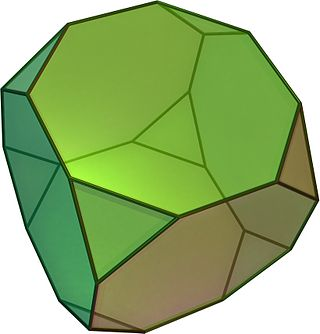
\includegraphics[width=2in]{TruncatedCube.jpg}
\end{center}
\caption{Truncated cube. [Image source: \href{https://en.wikipedia.org/wiki/Truncated_cube}{Wikipedia}]}\label{fig:TruncatedCube}
\end{figure}

It turns out that the subgroups of symmetric groups play an important role in group theory.

\begin{definition}
Every subgroup of a symmetric group is called a \textbf{permutation group}.
\end{definition}

The proof of the following theorem isn't too bad, but we'll take it for granted. After tinkering with a few examples, you should have enough intuition to see why the theorem is true and how a possible proof might go.

\begin{theorem}[Cayley's Theorem]
Every finite group is isomorphic to some permutation group.  In particular, if $G$ is a group of order $n$, then $G$ is isomorphic to a subgroup of $S_n$.
\end{theorem}

Cayley's Theorem guarantees that every finite group is isomorphic to a permutation group and it turns out that there is a rather simple algorithm for constructing the corresponding permutation group.  I'll briefly explain an example and then let you try a couple.

Consider the Klein four-group $V_4=\{e,v,h,vh\}$.  Recall that $V_4$ has the following group table.

\begin{center}
\begin{tabular}{c!{\vrule width 2pt}c|c|c|c}
$*$ & $e$ & $v$ & $h$ & $vh$ \\ \noalign{\hrule height 2pt}
$e$ & $e$ & $v$ & $h$ & $vh$ \\
\hline $v$ & $v$ & $e$ & $vh$ & $h$  \\
\hline $h$ & $h$ & $vh$ & $e$ & $v$\\
\hline $vh$ & $vh$ & $h$ & $v$ & $e$
\end{tabular}
\end{center}

If we number the elements $e,v,h,$ and $vh$ as $1,2,3,$ and $4$, respectively, then we obtain the following table.

\begin{center}
\begin{tabular}{c!{\vrule width 2pt}c|c|c|c}
 & $1$ & $2$ & $3$ & $4$ \\ \noalign{\hrule height 2pt}
$1$ & $1$ & $2$ & $3$ & $4$ \\
\hline $2$ & $2$ & $1$ & $4$ & $3$  \\
\hline $3$ & $3$ & $4$ & $1$ & $2$\\
\hline $4$ & $4$ & $3$ & $2$ & $1$
\end{tabular}
\end{center}

\noindent Comparing each of the four columns to the leftmost column, we can obtain the corresponding permutations.  In particular, we obtain
\begin{align*}
e&\leftrightarrow (1)\\
v&\leftrightarrow (1,2)(3,4)\\
h&\leftrightarrow (1,3)(2,4)\\
vh&\leftrightarrow(1,4)(2,3). 
\end{align*}
Do you see where these permutations came from?  The claim is that the set of permutations $\{(1),(1,2)(3,4),(1,3)(2,4),(1,4)(2,3)\}$ is isomorphic to $V_4$.  In this particular case, it's fairly clear that this is true.  However, it takes some work to prove that this process will always result in an isomorphic permutation group.  In fact, verifying the algorithm is essentially the proof of Cayley's Theorem. 

Since there are potentially many ways to rearrange the rows and columns of a given table, it should be clear that there are potentially many isomorphisms that could result from the algorithm described above.

Here's another way to obtain a permutation group that is isomorphic to a given group.  Let's consider $V_4$ again.  Recall that $V_4$ is a subset of $D_4$, which is the symmetry group for a square.  Alternatively, $V_4$ is the symmetry group for a non-square rectangle.  Label the corners of the rectangle 1, 2, 3, and 4 by starting in the upper left corner and continuing clockwise.  Recall that $v$ is the action that reflects the rectangle over the vertical midline.  The result of this action is that the corners labeled by 1 and 2 switch places and the corners labeled by 3 and 4 switch places.  Thus, $v$ corresponds to the permutation $(1,2)(3,4)$.  Similarly, $h$ swaps the corners labeled by 1 and 4 and the corners labeled by 2 and 3, and so $h$ corresponds to the permutation $(1,4)(2,3)$.  Notice that this is not the same answer we got earlier and that's okay as there may be many permutation representations for a given group.  Lastly, $vh$ rotates the rectangle $180^{\circ}$ which sends ends up swapping corners labeled 1 and 3 and swapping corners labeled by 2 and 4.  Therefore, $vh$ corresponds to the permutation $(1,3)(2,4)$.

\begin{problem}
Consider $D_4$.
\begin{enumerate}[label=\rm{(\alph*)}]
\item Using the method outlined above, find a subgroup of $S_8$ that is isomorphic to $D_4$.
\item Label the corners of a square 1--4. Find a subgroup of $S_4$ that is isomorphic to $D_4$ by considering the natural action of $D_4$ on the labels on the corners of the square.
\end{enumerate}
\end{problem}

\begin{problem}
Consider $\mathbb{Z}_6$.
\begin{enumerate}[label=\rm{(\alph*)}]
\item Using the method outlined earlier, find a subgroup of $S_6$ that is isomorphic to $\mathbb{Z}_6$.
\item Label the corners of a regular hexagon 1--6. Find a subgroup of $S_6$ that is isomorphic to $\mathbb{Z}_6$ by considering the natural action of $\mathbb{Z}_6$ on the labels on the corners of the hexagon.
\end{enumerate}
\end{problem}

\end{section}

\begin{section}{Alternating Groups}

In this section, we describe a special class of permutation groups.  To get started, let's play with a few exercises.

\begin{problem}
Write down every permutation in $S_3$ as a product of 2-cycles in the most efficient way you can find (i.e., use the fewest possible transpositions).  Now, write every permutation in $S_3$ as a product of adjacent 2-cycles, but don't worry about whether your decompositions are efficient.  Any observations about the number of transpositions you used in each case?  Think about even versus odd.
\end{problem}

\begin{lemma}
If $\alpha_1,\alpha_2,\ldots,\alpha_k$ is a collection of 2-cycles in $S_n$ such that $\alpha_1\alpha_2\cdots\alpha_k=(1)$, then $k$ must be even.
\end{lemma}

\begin{proof}
Suppose $\alpha_1,\alpha_2,\ldots,\alpha_k$ is a collection of 2-cycles in $S_n$ such that $\alpha_1\alpha_2\cdots\alpha_k=(1)$.  We need to show that $k$ is even. We proceed by strong induction. First, it is clear that the statement is not true when $k=1$, but is true when $k=2$. 

Now, assume that $k>2$ and if $j\leq k-1$ and we have a product of $j$ 2-cycles that equals the identity, then $j$ is even. Consider $\alpha_1\alpha_2$. The only possibilities are:
\begin{enumerate}
\item[(i)] $\alpha_1\alpha_2=(a,b)(a,b)$,
\item[(ii)] $\alpha_1\alpha_2=(a,b)(a,c)$,
\item[(iii)] $\alpha_1\alpha_2=(a,b)(c,d)$,
\item[(iv)] $\alpha_1\alpha_2=(a,b)(b,c)$.
\end{enumerate}
If case (i) happens, then
\[
(1)=\alpha_1\alpha_2\cdots,\alpha_k=\alpha_3\alpha_4\cdots\alpha_k.
\]
Since the expression on the right consists of $k-2$ factors, $k-2$ must be even by induction, which implies that $k$ is even. Now, suppose we are in one of cases (ii), (iii), or (iv). Observe that:
\begin{enumerate}
\item[(ii)] $(a,b)(a,c)=(b,c)(a,b)$,
\item[(iii)] $(a,b)(c,d)=(c,d)(a,b)$,
\item[(iv)] $(a,b)(b,c)=(b,c)(a,c)$.
\end{enumerate}
In each case, we were able to move $a$ from the original left 2-cycle to a new right 2-cycle. That is, we were able to rewrite $\alpha_1\alpha_2$ so that $a$ does not appear in the left 2-cycle. Systematically repeat this process for the pairs $\alpha_2\alpha_3$, $\alpha_3\alpha_4$,\ldots, $\alpha_{k-1}\alpha_k$. If we ever encounter case (i) along the way, then we are done by induction. Otherwise, we are able to rewrite $\alpha_1\alpha_2\cdots\alpha_k$ so that $a$ only appears in the rightmost 2-cycle. But this implies that $\alpha_1\alpha_2\cdots\alpha_k$ does not fix $a$, which contradicts $\alpha_1\alpha_2\cdots\alpha_k =(1)$. This implies that at some point we must encounter case (i), and hence $k$ is even by induction.
\end{proof}

\begin{theorem}
If $\sigma\in S_n$, then every transposition representation of $\sigma$ has the same parity.
\end{theorem}

The previous theorem tells us that the following definition is well-defined.

\begin{definition}
A permutation is \textbf{even} (respectively, \textbf{odd}) if one of its transposition representations consists of an even (respectively, odd) number of transpositions.
\end{definition}

\begin{problem}
Classify all of the permutations in $S_3$ as even or odd.
\end{problem}

\begin{problem}
Classify all of the permutations in $S_4$ as even or odd.
\end{problem}

\begin{problem}
Determine whether $(1,4,2,3,5)$ is even or odd.  How about $(1,4,2,3,5)(7,9)$?
\end{problem}

\begin{problem}
Consider the arbitrary $k$-cycle $(a_1,a_2,\ldots, a_k)$ from $S_n$ (with $k\leq n$).  When will this cycle be odd versus even?  Briefly justify your answer. 
\end{problem}

\begin{problem}
Conjecture a statement about when a permutation will be even versus odd.  Briefly justify your answer.
\end{problem}

And finally, we are ready to introduce the alternating groups.

\begin{definition}
The set of all even permutations in $S_n$ is denoted by $A_n$ and is called the \textbf{alternating group}.
\end{definition}

Since we referred to $A_n$ as a group, it darn well better be a group!

\begin{theorem}
The set $A_n$ forms a group under composition of permutations and has order $n!/2$.\footnote{\emph{Hint:} To show that $A_n$ is a group, argue that $A_n$ is a subgroup of $S_n$ using the Two-Step Subgroup Test (see Theorem~\ref{thm:subgroup_criterion}). To show that $|A_n|=n!/2$, prove that the number of even permutations in $S_n$ is the same as the number of odd permutations in $S_n$.  Here is one way to accomplish this. Define $f:S_n\to S_n\setminus A_n$ via $f(\sigma)=(1,2)\sigma$.  Note that $S_n\setminus A_n$ is the set of odd permutations in $S_n$. Show that $f$ is a bijection.}
\end{theorem}

\begin{problem}
Find $A_3$.  What group is $A_3$ isomorphic to?
\end{problem}

\begin{problem}
Find $A_4$ and then draw its subgroup lattice. Is $A_4$ abelian?
\end{problem}

\begin{problem}
What is the order of $A_5$?  Is $A_5$ abelian?
\end{problem}

\begin{problem}
What are the possible orders for elements in $S_6$ and $A_6$?  What about $S_7$ and $A_7$?
\end{problem}

\begin{problem}
Does $A_8$ contain an element of order 15?  If so, find one.  If not, explain why no such element exists.
\end{problem}

\begin{remark}
Below are a few interesting facts about $A_4$ and $A_5$, which we will state without proof.
\begin{enumerate}[label=\rm{(\alph*)}]
\item The group of rigid motion symmetries for a regular tetrahedron is isomorphic to $A_4$.
\item You can arrange the Cayley diagram for $A_4$ with generators $(1,2)(3,4)$ and $(2,3,4)$ on a truncated tetrahedron, which is depicted in Figure~\ref{fig:TruncatedTetrahedron}.
\item You can arrange the Cayley diagram for $A_5$ with generators $(1,2)(3,4)$ and $(1,2,3,4,5)$ on a truncated icosahedron, which is given in Figure~\ref{fig:TruncatedIcosahedron}.  You can also arrange the Cayley diagram for $A_5$ with generators $(1,2,3)$ and $(1,5)(2,4)$ on a truncated dodecahedron seen in Figure~\ref{fig:TruncatedDodecahedron}. 
\end{enumerate}
\end{remark}

\begin{figure}[!ht]
\begin{center}
\subcaptionbox{\label{fig:TruncatedTetrahedron}}[.3\textwidth]{
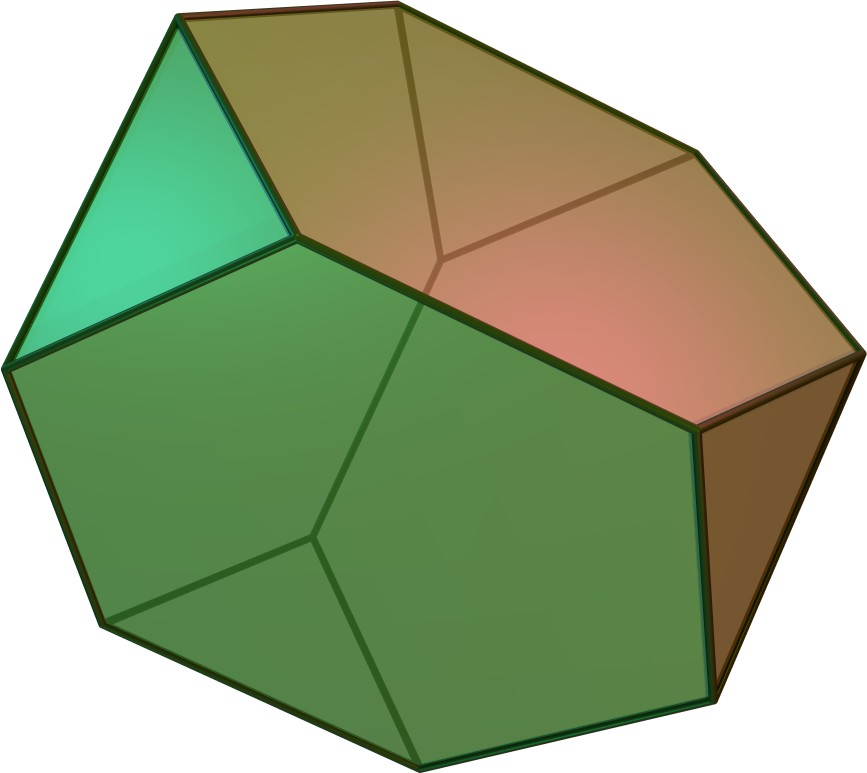
\includegraphics[width=1.5in]{TruncatedTetrahedron}
}
\subcaptionbox{\label{fig:TruncatedIcosahedron}}[.3\textwidth]{
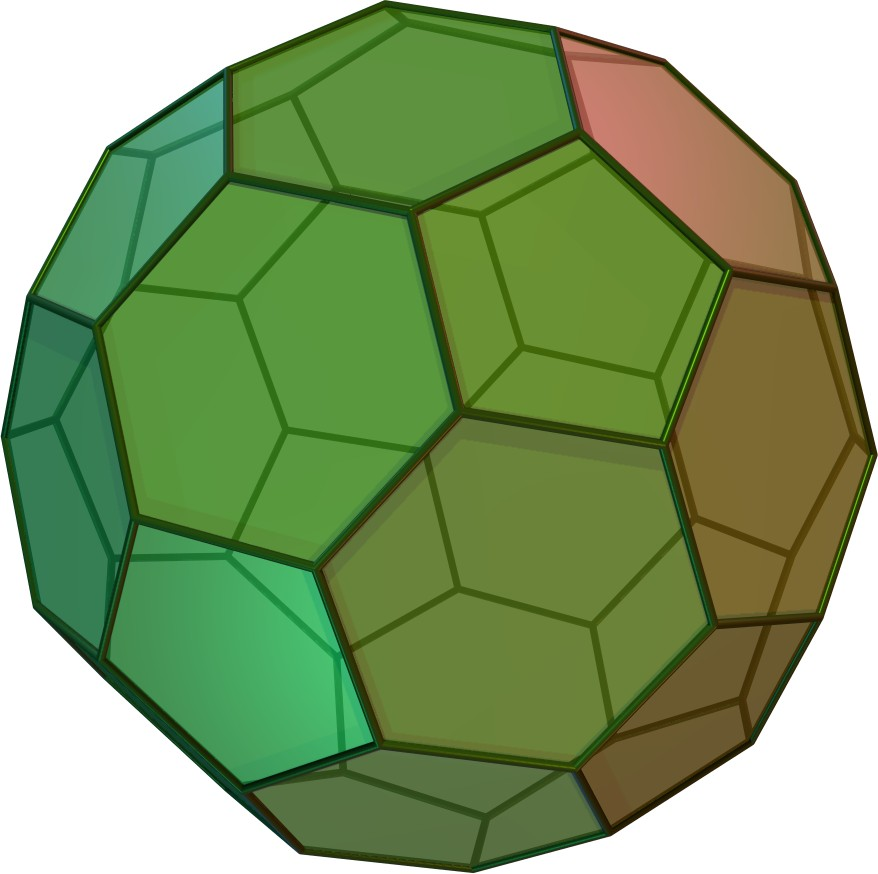
\includegraphics[width=1.5in]{TruncatedIcosahedron}}
\subcaptionbox{\label{fig:TruncatedDodecahedron}}[.3\textwidth]{
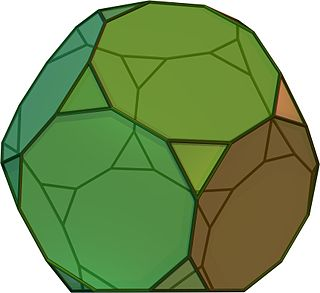
\includegraphics[width=1.5in]{TruncatedDodecahedron}}
\caption{Truncated tetrahedron, truncated icosahedron, and truncated dodecahedron. [Image source: \href{https://en.wikipedia.org/wiki/Truncated_tetrahedron}{Wikipedia}]}
\end{center}
\end{figure}

\end{section}